\documentclass{article}
\usepackage{graphicx}
\usepackage{float}

\begin{document}
    \title{
        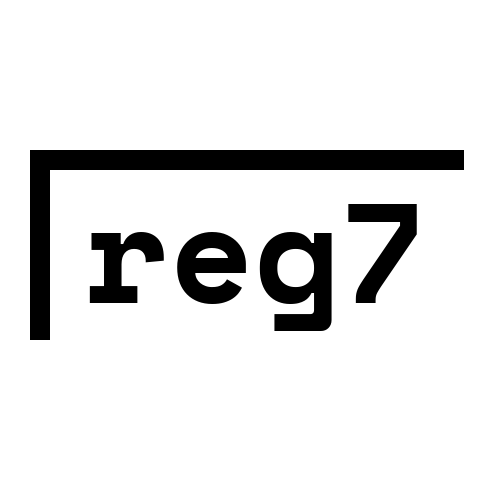
\includegraphics[width=0.5\textwidth]{./logo.png} \\[2cm]
        Fonctionnalités de l'application
    }
    \author{Alexandre Trotel, Ayoub Bouchama, Clément Cognard, \\Clément Safer, Ewen Le Bihan, Florent Puy, \\Gauthier Rancoule, Ilyasse Alioui, Raphaël Giudice}
    \date{Lundi 26 Février 2023}

    \maketitle
    \newpage

    \section{Objectif général}

    Cette application vise à démystifier les expressions régulières, et à faciliter leur apprentissage grâce à une approche visuelle par blocs, testée sur le terrain par des acteurs reconnus par l'Éducation Nationale, tels que \emph{Scratch}.

    Mais, à la différence de \emph{Scratch}, on n'oublie pas la réalité des expressions régulières, en plaçant également en premier plan la vraie expression régulière, ce qui permet à l'apprenant d'utiliser ses compétences pour dans le futur lire et écrire ses propres expressions simples sans avoir besoin d'un logiciel tiers.

    Cette application pourra également servir à des programmeurs expérimentés qui souhaitent comprendre une expression particulièrement complexe, et en tester son fonctionnement simplement.

    \section{Fonctionnalités attendues}

    \begin{description}
        \item[Analyse d'expressions régulières] Notre application doit être capable d'analyser des expressions régulières pour déterminer leur validité et leur structure syntaxique. Nous allons essayer d’inclure des fonctionnalités telles que la coloration syntaxique et la mise en évidence des erreurs pour aider les utilisateurs à comprendre leur expression régulière.
Celle-ci est une fonctionnalité clé de tout logiciel qui traite les expressions régulières. Elle permet à l'utilisateur de vérifier la validité de l'expression régulière qu'il a saisie et de détecter les erreurs de syntaxe éventuelles. En effet, la syntaxe des expressions régulières peut être complexe et difficile à comprendre pour les débutants. L'importance de cette fonctionnalité réside dans le fait qu'elle permet à l'utilisateur de gagner du temps en détectant les erreurs de syntaxe dès la saisie de l'expression régulière. Elle permet également d'améliorer la qualité du code en évitant les erreurs de syntaxe et de faciliter l'apprentissage des expressions régulières pour les débutants.

\item[Construction d'expressions régulières] Notre application devrait permettre à l'utilisateur de construire des expressions régulières à partir de blocs de construction prédéfinis,
tels que des classes de caractères, des quantificateurs et des groupes de capture. Les utilisateurs peuvent également bénéficier des outils d'auto complétion pour faciliter la construction. Cette fonctionnalité est importante car elle permet aux utilisateurs de créer des expressions régulières complexes sans avoir à se soucier de la syntaxe et de la structure de l'expression régulière. Cela peut aider les utilisateurs à gagner du temps et à éviter les erreurs syntaxiques courantes. En outre, elle facilite l'apprentissage des expressions régulières pour les débutants en leur fournissant des blocs de construction prédéfinis qu'ils peuvent utiliser comme point de départ pour construire des expressions régulières plus complexes.

\item[Test d'expressions régulières] Notre application devrait permettre aux utilisateurs de tester leurs expressions régulières en les appliquant à des chaînes de texte pour voir si elles correspondent ou non. Nous allons également essayer d’inclure des outils pour explorer les résultats de match et de capture. La fonctionnalité de test d'expressions régulières est importante car elle permet aux utilisateurs de vérifier si leurs expressions régulières correspondent ou non à une chaîne de texte spécifique. Cela permet aux utilisateurs de s'assurer que leur expression régulière fonctionne comme prévu avant de l'appliquer à une application ou un programme plus large. Les résultats de match indiquent si l'expression régulière correspond ou non à la chaîne de texte, tandis que les résultats de capture permettent aux utilisateurs d'extraire des sous-chaînes spécifiques qui correspondent à des parties de l'expression régulière. La visualisation des résultats de match et de capture peut aider les utilisateurs à comprendre comment leur expression régulière fonctionne et à trouver des erreurs ou des problèmes potentiels. Cela peut également aider les utilisateurs à développer des expressions régulières plus efficaces en leur permettant de voir les parties de la chaîne de texte qui correspondent et celles qui ne correspondent pas.

\item[Exportation d'expressions régulières] Notre application doit permettre aux utilisateurs d'exporter leurs expressions régulières sous forme de code Java, de code Python, de code Perl ou d'autres langages de programmation. Cette fonctionnalité est importante car elle permet à l'utilisateur de réutiliser facilement leur expression régulière dans d'autres programmes ou projets, sans avoir à la saisir à nouveau.
En effet, la saisie d'une expression régulière peut être fastidieuse et complexe, et l'exportation de l'expression régulière sous forme de code permet à l'utilisateur de gagner du temps et de minimiser les erreurs. Cette fonctionnalité est également utile pour les développeurs qui travaillent dans plusieurs langages de programmation, car ils peuvent facilement exporter l'expression régulière dans le langage qu'ils utilisent.
En outre, l'exportation d'expressions régulières peut être un outil pédagogique utile pour les apprenants en programmation qui peuvent analyser le code généré pour comprendre comment les expressions régulières fonctionnent et comment les utiliser efficacement.

\item[L'importation d'expressions régulières]  C’est une fonctionnalité importante pour toute application de traitement de texte. Elle permet aux utilisateurs d'importer des expressions régulières qu'ils ont déjà créées et sauvegardées ailleurs, plutôt que de devoir les saisir à nouveau manuellement. La fonctionnalité d'importation d'expressions régulières peut également aider les débutants à apprendre à utiliser les expressions régulières en leur permettant d'importer des exemples existants et de les étudier. Elle peut également être utile pour les utilisateurs qui ne sont pas familiers avec la syntaxe d'un langage de programmation particulier, car elle leur permet d'importer des expressions régulières créées par des experts dans ce langage.

\item[Gestion de l'historique] Notre application va permettre aux utilisateurs de revenir en arrière et de refaire des modifications à leur expression régulière. Nous allons essayer également d’ inclure des outils pour enregistrer l'historique des modifications et permettre aux utilisateurs de parcourir leur historique pour trouver des versions antérieures.

\item[Didactiel] Notre application comprendra également un tutoriel guidé destiné aux débutants pour les aider à comprendre les expressions régulières. Ce tutoriel fournira une introduction aux expressions régulières, expliquera leur importance et présentera les principales bases à retenir pour les utiliser efficacement. Il guidera l'utilisateur à travers des exemples simples et les aidera à comprendre les concepts fondamentaux tels que les caractères spéciaux, les classes de caractères et les quantificateurs. Le tutoriel fournira également des conseils pratiques pour la création d'expressions régulières efficaces et aidera les utilisateurs à éviter les erreurs courantes. En bref, ce didacticiel permettra aux débutants de se familiariser avec les expressions régulières et de commencer à les utiliser de manière efficace dans leur travail quotidien.
    \end{description}

    \section{Interface utilisateur envisagée}
    \begin{figure}[H]
        \centering
        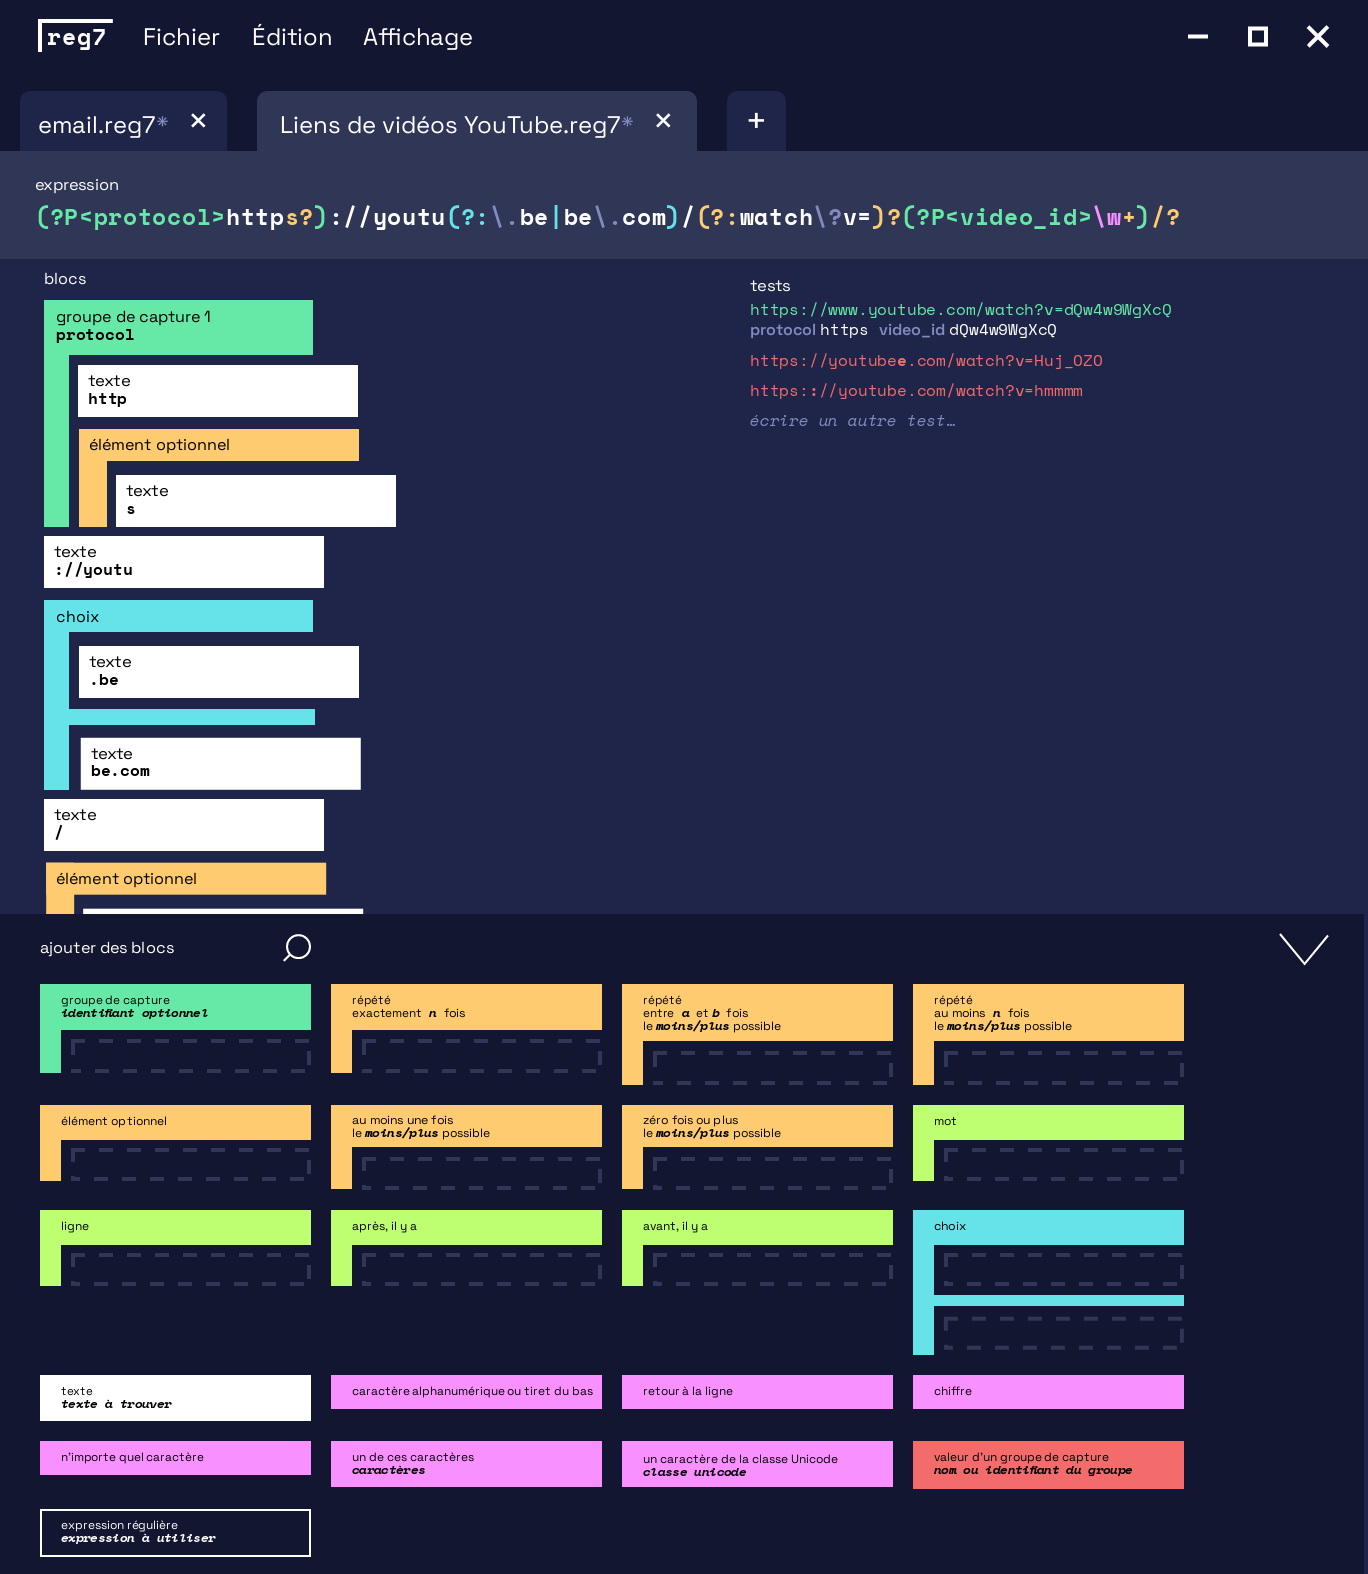
\includegraphics[width=0.9\textwidth]{prototype.png}
        \caption{Prototype de l'interface utilisateur}
        \label{fig:prototype}
    \end{figure}

    Nous envisageons une inteface en cinq parties
    \begin{description}
        \item[le \emph{header} ] contrôles de fenêtre, les menus Fichier, Edition et Affichage, et les onglets.
            \item[expression] L'expression régulière générée par les blocs, avec une coloration syntaxique cohérente aux couleurs des différents blocs

            \item[blocs] l'expression régulière représentée sous forme d'imbrication de blocs, que l'on peut réorganiser et supprimer, à la \emph{Scratch}.

                \item[tests] chaque ligne est une valeur concrète sur laquelle tester l'expression régulière.
                    Les valeurs qui ne vérifient pas l'expression sont en rouge, celles la vérifiant sont en vert, avec les valeurs des groupes de capture affichées (si le groupe de capture n'a pas de nom, on utilise son numéro)

\item[ajouter des blocs] Une section que l'on peut réduire, contenant les différents blocs que l'on peut faire glisser dans la section \emph{blocs} .
    \end{description}
    
    \section{Cas d'usage}
    \paragraph{}
    
    Les expressions rationnelles sont aujourd’hui omniprésentes dans l’univers  numérique. Cependant, la construction de telles expressions est souvent effrayante et difficilement accessible au grand public. Notre idée est de simplifier cette étape de la construction grâce à une interface simple et intuitive. Le programmeur lambda pourra ainsi construire ses propres expressions et les utiliser. 

    \paragraph{}
    Il pourra par exemple, pour remplir un champ sur un  site, exiger une réponse conforme (ne vouloir que des réponses correspondant à la syntaxe d’une adresse mail ou d’un numéro de téléphone français). 

    \paragraph{}
    Il pourra également filtrer ou regrouper du contenu aisément, le tout depuis une interface intuitive permettant la construction par bloc et l’analyse de l’expression sur place.
    
\end{document}
